\documentclass[preprint,3p,times,twocolumn]{elsarticle}
\usepackage{amssymb}
\usepackage{amsmath} %for equation
\usepackage{footnote} %for footnote
%\usepackage{hyperref}
\usepackage{lineno}
\usepackage{colortbl}
\usepackage[pdftex,dvipsnames]{xcolor}
\newcommand{\Rim}[1]{\textcolor{Green}{#1}}
\usepackage[framemethod=tikz]{mdframed}
\usepackage{multirow}
%\usepackage{hyperref} %for url

\begin{document}
\linenumbers
\begin{frontmatter}
\title{Variable spraying control using model-checking}


\author[inst1]{Rim Saddem-Yagoubi}
\author[inst3]{Anice Cheraiet}

\author[inst2]{Karen Godary-Dejean}
\author[inst2]{Didier Crestani}
\author[inst3]{Olivier Naud}
\affiliation[inst1]{organization={LIS, Aix-Marseille University, CNRS },
            addressline={52 Av. Escadrille Normandie Niemen}, 
            city={Marseille},
            postcode={13397},
            country={FRANCE}}

\affiliation[inst2]{organization={LIRMM UMR 5506 CNRS, Univ Montpellier},%Department and Organization
            addressline={161 rue Ada}, 
            city={Montpellier},
            postcode={34392}, 
            country={FRANCE}}

\affiliation[inst3]{organization={ITAP, Univ Montpellier, INRAE, Institut Agro},%Department and Organization
            %addressline={361 rue Jean-François Breton}, 
            city={Montpellier},
            %postcode={34196}, 
            state={France}}
         
\begin{abstract}
	%% Text of abstract
	One major challenge for agriculture is the sustainable use of pesticides. Once a treatment is deemed necessary, reducing overall sprayed quantities while ensuring required protection to each plant is a major direction for precision agriculture technologies in crop protection. In this paper, a new planning method for Variable Rate Application (VRA) called AMPS (Automata Modelling for Precision Spraying) is presented. It was designed to allow optimising sprayed crop protection products based on canopy density data and recommendations on appropriate spraying commands depending on this data. The new method considers constraints on the sprayer actuators (behaviour, dynamics), and use formal methods (model checking and CORA - Cost Optimal Reachability Analysis algorithm) to find the guaranteed optimised value for spraying a field. As formal methods are well known to have issues with regards to combinatorics, a decomposition methodology is proposed, that uses the specific spatialised characteristic of crops to simplify the modelling and analysis steps. The AMPS methodology is applied to a grapevine case using LiDAR data for characterising vegetation density.  The conclusion presents the advances and limitations of this work and suggests ways to improve. Other applications of model-checking in agriculture are also suggested.
\end{abstract}

\begin{keyword}
	
	Precision spraying \sep Model-checking \sep Cost-Optimal Reachability Analysis   \sep Formal verification \sep Controller
	synthesis  \sep   UPPAAL-CORA  \sep  Optimisation 
\end{keyword}

\end{frontmatter}



\section{Introduction}
\label{intro}
The current challenge for agriculture is to improve the quality and quantity of products while preserving the human health and the environment. One of the ways to meet this challenge is to use Precision Agriculture technologies. Precision agriculture has for origin the development of localisation and sensing technologies by which site specific management can be implemented in the field, in order to optimise a given criterion, e.g. economical or environmental benefit \cite{BERK2016273}. Most recent technologies like multi-spectral imagery and laser scanning, whether airborne or from the ground, allow the acquisition of crop data with a high spatial resolution \cite{rosell2009obtaining}, \cite{hall2003characterising}. On both arable and perennial crops, sensors can be used to quantify and map the dimensional and density characteristics of vegetation (\cite{Michaud200829}). This spatial information is an opportunity for automation specialists to develop innovative and efficient methods for accurate site specific agricultural action using Variable Rate Application (VRA, \cite{gil2007variable}) Technologies (VRT). VRT enable optimisation of inputs (fertilisers, amendments, water, pesticides, etc) with regard to outputs (yield, quality of the product, quality of the environment, profits, etc). 

Over the last two decades, VRA as applied to spraying of crop protection products has received growing attention from scientists and seen the production of commercial systems for various crops. This is the case for orchards and vineyards\cite{wandkar2018}.

VRA as of today is mainly enacted according to two alternative application principles. The first principle can be called \textit{real-time} or \textit{on-the-go} VRA. According to this principle, a measurement is done on the crop or on the soil and the rate of application of the agricultural input is modified in real-time according to a set of calculations. Most often, the measurement is a single measurement and the output of the control is also a single one: the rate of application of the agricultural input. Usually, no feedback needs to be implemented on variable rate control. This is because, thinking time on a discrete scale, the action of the machinery at $t+1$ is not made on the same location as where the action at $t$ was made. Thus, in control science terminology, real-time VRA is most often single-input single-output open loop control.

The second principle is VRA according to a recommendation or prescription map. In this case, the recommendation map is prepared according to geo-localised information previously acquired. Usually, a map is calculated according to local variations of a given agronomic attribute. So-called "decision rules" are applied. Most often, the quantitative decision rules are based on a linear model. The farmer may have access to parameters to tune the recommendation map and to editing features to override values on the map. Considering high resolution site specific action, one key element is often missing: the behaviour and precision of actuators. This has been recognised in works such as \cite{roudier2011TOI} in which the influence of spatial footprint of machinery and of uncertainty of actual output with regard to prescribed setpoint are highlighted. One key point is the time of reaction, which influences spatial precision along the machine track \cite{Chan2004601}, depending on machine speed. Thus, reaction time and machine behaviour may hinder the proper application of a recommendation map that would be solely based on characteristics of the vegetation. This is why one may think about an alternative approach to recommendation maps: maps with predefined and geo-referenced control set-points (here: spraying configurations and flow rates). Such set-points may be defined by an expert according to rules about vegetation and constraints of the sprayer. A control theory can be use to manage these control set-points for automated devices using numerical control. For example, the model-checking. The purpose of model-checking here is to verify that a desired state of a system can be reached, and it can provide a sequence of set-points allowing to reach this desired state. Furthermore, using Cost Optimal Reachability Analysis (CORA), a sequence that is optimised according to a given cost can be provided.

In this paper, the possibility to use model-checking and CORA to compute an optimised control sequence for sprayers in a vineyard is investigated.

More specifically, considering the control dynamics of a sprayer and the possibility to acquire LiDAR data that characterise the vegetation before spraying, a precision agriculture oriented method that computes an optimal spray command sequence is proposed. The proposed method includes a decomposition technique to leverage the combinatorial explosion issues that are commonly encountered when performing model-checking.
An assessment of this method based on LiDAR data acquired in vineyards in the south of France is provided.

This paper builds on previously published research \cite{saddem2017jai} with new extensive explanations on modelling, new assessment based on full-scale field data, and a key algorithmic feature required to solve real-world agricultural problems with model-checking: a decomposition method. The outline of the paper is as follows. Section 2 describes the study context. Section 3 details the Automata Modelling for Precision Spraying (AMPS) method. Section 4 is devoted to the decomposition method. In Section 5, experimental results are described and discussed before concluding.
%%%%%%%%%%%%%%%%%%%%%%%%%%%%%%%%%%%%%%%%%%%%%%%%%%%%%%%%%%%%%%%%%%%%%%%%%%%%%%%%%%%%%%%%%%%%%%%%%%%%%%%%%%%%%%%%%%%%%%%%%%%%%%%%%%%%%%%%%%%%%
%%%%%%%%%%%%%%%%%%%%%%%%%%%%%%%%%%%%%%%%%%%%%%%%%%%%%%%%%%%%%%%%%%%%%%%%%%%%%%%%%%%%%%%%%%%%%%%%%%%%%%%%%%%%%%%%%%%%%%%%%%%%%%%%%%%%%%%%%%%%%
\section{Background and study context}
A short background on model-checking and tooling for cost optimal reachability analysis is provided in the beginning of this section. Details of the precision spraying problem to solve are then given. The proposed general methodology, named AMPS, is described in the following section.
%the technical context of the study is presented, describing the main concepts and tools necessary to understand our work.


\subsection{Model-checking}
\indent The Model-Checking (MC) was introduced in the early 1980s \cite{MCSifakis}, \cite{clarke1981design}. It provides formal verification methods to ensure that the model of a system conforms to its specifications. It is usually used to analyse communications protocols \cite{duflot2012practical} or industrial applications \cite{clabaut2016industrial}, \cite{Transformation2020}, \cite{IndustrieMC}.
\subsubsection{Model-checking phases}
\label{MC}

The model-checking process is based on 3 phases, namely modelling, specification and verification.
\paragraph{\textbf{The formal modelling phase}} $ \\ $
This phase consists in the formal modelling of the system behaviour. It is mainly based on state machines. States are an abstraction of the status of the system, while the transitions represent events making the system switch from one state to another. For timed systems, temporal constraints can be added to the model. The most popular formalisms for timed systems modelling are Timed Automata (TA) \cite{alur1990automata} and Time Petri nets \cite{berthomieu1991modelling}.

\paragraph{\textbf{The specification phase}} $ \\ $
The specification phase consists in describing the expected system specification using properties. These properties are expressed in logical languages such as LTL (Linear Temporal Logic) or CTL (Computation Tree Logic)~\cite{MC_BaierKatoen}. The properties defined for model checking~\cite{MC_BaierKatoen} are classically: invariants, safety, absence of deadlock, liveness, state (un)reachability.

\paragraph{\textbf{The verification phase}} $ \\ $
The verification phase consists in determining if the model satisfies the specified properties using a model-checking algorithm. First, the state graph containing all the possible reachable states is constructed. Then, this state space is explored, checking the satisfaction of the properties. Model checkers can record a diagnostic trace of the verification process along an execution path, from the initial state until the property is (un)satisfied.
Tools for model-checking can be classified in four categories: code analysis model-checkers, probabilistic model-checkers, ordinary model-checkers and timed model-checkers. A large and detailed comparison of the performance of many formal verification environments in checking a safety property has been made in \cite{mazzanti2018ten} and has shown that UppAAL is a reference tool.

UppAAL \footnote{https://uppaal.org/} is a tool chain designed to validate systems modelled as networks of timed automata. It extends the TA formalism by adding integer variables, structured data types, user defined functions, and synchronisation channels \cite{bengtsson2003timed}. The model checker of UppAAL allows to verify properties on the model of a system, analysing its state space. TA and UppAAL have already been used in the agricultural and ecosystem management domains (e.g. in \cite{dusseux2015paturmata}, \cite{largouet:2012}). 

Concurrently with the model-checking verification phase, an optimisation process can be carried out using Cost Optimal Reachability Analysis.

\subsubsection {\textbf{Model Checking and Cost Optimal Reachability Analysis (CORA)}} $ \\ $
\indent The notion of optimal cost is often used in scheduling and planning problems. Usually, constraints programming or linear programming approaches are used to solve such problems. The AMETIST project \cite{revised2006ametist} proposed in 2006 addresses these issues using model checking and proves the practical applicability of model checking tools. However, basic MC algorithms do not include the ability to find an execution path that verifies at the same time a property and its optimality according to a cost criterion chosen by a user. A variant of UppAAL called UppAAL-CORA \cite{priced2004} \cite{behrmann2005optimal} can provide a Cost Optimal Reachability Analysis. It addresses the problem of finding the minimum cost to reach a goal state.  It has been successfully used for solving various scheduling and routing problems (\cite{priced2004} including precision spraying \cite{saddem2017jai} or harvest optimisation problems (\cite{saddem2020model}, \cite{yagoubi2018new})).

The CORA algorithm is based on the branch and bound concept. Depending on the chosen branching strategy, it may explore the entire state space to find, among the set of attainable paths, an optimal cost path. The idea of the branching strategy \textit{"Minimum Cost order"} for reachability properties is to guide the exploration of the state space such that promising sets of states are visited first \cite{behrmann2001guiding}. For a given state, a partial cost is evaluated. Then globally, the state having the lowest partial cost is explored first. If the obtained state achieves the goal of reachability, then the path found is optimal. The so-called Remaining feature can be used to reduce the number of explored spaces and guide the exploration process \cite{priced2004}.

Since properties verification using model checking is based on state-space analysis, its main limitation concerns combinatorial explosion.

\subsubsection{Limit of Model Checking: The state space explosion problem}

State space explosion is a problem usually encountered during the verification phase of real systems. Its principal cause is the large size and the complexity of the model of the system to be verified. As MC enumerates exhaustively all the possible reachable states of a system, and stores them to verify properties, the combinatorial explosion affects both the time and space complexity of the verification algorithm. To deal with this problem, various techniques such as the reduction of the state space, the optimisation of modelling, or the limitation of the state space explored during the verification step, have been proposed

The most popular techniques for the reduction of state space are: 1) the binary decision diagram which provides a symbolic representation of states allowing a more compact representation of the state space \cite{burch1992symbolic}; 2) the partial order methods which consist in eliminating as much as possible unnecessary interlacing between parallel processes when constructing the state space (\cite{godefroid1996partial}, \cite{boucheneb2009covering}); and 3) the symmetry exploitation which is based on the exploitation of the structural symmetries of the system to build a reduced state space \cite{hendriks2003adding}.

For the optimisation of modelling, the choice of abstractions and simplifications influences greatly the size of the state space. However, the simplified models must guarantee the correctness of the verification of the properties. This requires expertise in the semantics of the modelling language, of the modelling process as well as in the underlying verification technique.

So-called on-the-fly algorithms allow to verify some properties without building the entire state space, reducing the time and the memory used during the verification process. This reduction is only effective for properties which do not require to explore the whole state space (like reachability ones). These algorithms are also useful to detect property violation (invariant, safety) since the first state that does not satisfy the property stops the verification process.

This sub-section summarised the basics of model checking and of the CORA techniques. Combinatorial explosion issues were pointed out as well as solutions to address them. 
The next section presents, in the context of precision agriculture, the Precision Spraying problem on which Model Checking, optimisation cost analysis and combinatorial explosion limitation methods are applied on.

\subsection{Detailed definition of the Precision Spraying Problem}

The spraying problem definition includes the spraying hardware involved, the constraints that need to be defined to guarantee local quality of spraying, and the objective for optimisation.

\subsubsection{Sprayer description}
\label{sec:Sprayer_Description}

In this section, a brief overview on different types of existing sprayers available for widely-spaced (wide inter-rows) vines is given. The hypothetical digitally controlled sprayer considered for the study is then presented.

\paragraph{\textbf{Presentation of a classic pneumatic sprayer}} $ \\ $
There are several types of sprayers that can be mounted on or trailed by a tractor: first treatment booms (having nozzles and no air assistance), airblast sprayers (nozzles mounted around a fan that generates the "airblast" that carries the droplet to canopy), pneumatic arches and pneumatic face to face sprayers, face to face sprayers with nozzles and air-assistance that can be turned off at early growth stages. Face to face sprayers can have recovery panels that recycle the spray that is not deposited in the canopy. In pneumatic sprayers, the air is used both to break the liquid into droplets and to carry the droplets obtained into the canopy. In figure \ref{fig:pulvecalvet} presented an example of a pneumatic arch type sprayer.

This sprayer has 4 spraying devices: a low hand (LH), a high hand (HH), a high cannon (HC) and a low cannon (LC). A "hand" is a spraying device comprising 2 or 3 nozzles, which will operate at the same time. When the sprayer is used, the hands spray on one side of the rows of vines adjacent to the sprayer. Cannons spray on distant rows of vines and can be arranged in various ways. In the following, to simplify the modelling and descriptions, only the hands of the sprayer will be considered.

\begin{figure}[h!]
\begin{center}
	\includegraphics[width=8cm]{sprayer.PNG}    
	\caption{Schematic representation in back view of a 4-handed, 4-cannon pneumatic arch with a low hand (LH), a high hand (HH), a high cannon (HC) and a low cannon (LC) } 
	\label{fig:pulvecalvet}
\end{center}
\end{figure}

\paragraph{\textbf{Hypothetical automated sprayer description}} $ \\ $
In general, pneumatic sprayers on the market do not have automatic mechanisms to independently close or open the spraying spouts in real time. The on-off switching of spouts is done manually.

In the example given in figure \ref{fig:pulvecalvet}, for example, both hands are typically used at the same time when vegetation is high enough. However, the automation of the control of individual spraying elements is essential for precision spraying. There are published examples of automated prototypes such as \cite{gil2007variable}, \cite{xiongkui2011precision}. 

To provide an example for the precision spraying methodology proposed in this paper, a hypothetical sprayer that can switch on/off each of its hands independently is proposed. In order to provide a mean to reduce the volume sprayed when vegetation is high but of a low foliage density, it is supposed that a third Central Hand, named CH, is added to the original Low Hand (LH) and High Hand (HH) (Figure \ref{fig:pulvecalvet}). CH is supposed designed and set to that it can cover approximately the same crop height as LH and HH used together. Spraying with the CH alone provides only half the volume that combined LH and HH provide. Indeed, each hand is supposed to have the same flow rate, which is half the nominal flow rate (the nominal flow means a full dose of the product).

The vertical position of each hand on the sprayer, its inclination, as well as its lateral distance from the vegetation define the height of vegetation it covers. One important aspect in the hypothetical sprayer considered is that opening and closing each hand takes some time.


In this article, for the sake of simplicity and genericity, we will call each "hand" of sprayer a “nozzle”, even if a "hand" actually comprises several spray sources operating simultaneously. Generally speaking, the principle proposed here is that redundant nozzles can be used to provide both adequate spray targeting as well as the optimal management of the dose to be applied. This principle can be applied to many types of sprayers. By redundant nozzles, it is meant that sprays of these nozzles may overlap in the height portion of the vegetation they cover.

\subsubsection{Precision Spraying Problem and constraints: A comprehensive definition}
\label{sec:Spraying_Constraints}

The Precision Spraying Problem consists in verifying the aptitude of an agricultural sprayer to respect the constraints of the task while, at the same time, providing an optimal sequence of sprayer commands. 

Spraying constraints can be classified into two categories: 1) Sprayer Constraints (SC) related to the dynamics of the agricultural machine, and 2) Agronomic Constraints (AC) which are related to requirements on precision spraying behaviour. 

In the context of the study, Sprayer Constraints are the speed of the sprayer (1.4 $m/s$), the number of nozzles (3), the orientation of the nozzles, the opening time of the nozzles (0.2 s) and the closing time of the nozzles (0.2 s). 
Agronomic Constraints are about spraying enough and with adequate vegetation targeting to protect each plant from disease. In this paper, AC rely on a Precision Spraying Mapping that stipulates which nozzles to use according to vegetation profile. This mapping is defined in section \ref{sec:AMPSmethodo}. Because it takes time to open and close valves, one rule is added to AC: when a new set point is required for the set of nozzles, the required nozzles should always be opened before closing the ones to shut down.
The agro-environmental objective is to minimise the total quantity of plant protection products sprayed in a field while respecting SC and AC.

More precisely, given a grapevine crop organised in rows, the objective of the Precision Spraying Problem (PSP) is to find a sequence of sprayer commands that sprays the entire crop while respecting all spraying constraints (SC and AC) and minimising the total quantity of sprayed product. 

To resolve PSP, a method called Automata Modelling for Precision Spraying (AMPS) has been designed. It is described in the next section.


\section{The AMPS methodology} 
\label{sec:AMPSmethodo}

This section presents the AMPS method for precision spraying.

\subsection{General description of AMPS}
The AMPS method takes 2D ground-based LiDAR data of the canopy as input. It then computes, for a given sprayer with individual control of nozzles, a command sequence optimised for a cost criterion while ensuring a sufficient protection on each vine plant. The flow rate and the response time for opening or closing the nozzles are parameters taken into account in the modelling as they will affect the choice of the most appropriate command for the sprayer.


AMPS is based on 3 steps, represented in figure \ref{fig:MethodoComplete}:
\begin{itemize}
\item [\textbf{Step 1:}] Define a static correspondence function between the vegetation density and the spray commands. This function, called "Precision Spraying Mapping" (PSM), maps each possible vegetation state to two spray commands: the most suitable command $C_{best}$, and an alternative acceptable command $C_{alt}$. These two commands guarantee sufficient protection for each vine plant. This step is based on human expertise about spraying and crop protection. The PSM may be tailored according to a grower's expertise and attitude towards its crop management. 
As the AMPS method is modular, steps 2 and 3 are not dependent on the PSM that is chosen.

\begin{figure}[ht!]
	%\begin{minipage}{2\linewidth}
	\begin{center}
		\includegraphics[width=7.7cm]{export.pdf}
		\caption{AMPS Method} 
		\label{fig:MethodoComplete}
	\end{center}
	%\end{minipage}
\end{figure}    
\item [\textbf{Step 2:}] Apply a data processing algorithm to raw LiDAR data from scans of vine rows. This algorithm produces for each row a Spatialised Recommendation Map (SRM). 
First, the algorithm uses aggregation and filtering rules to form blocks of vegetation which have a uniform vegetation density. The length of each block can vary from one block to another, with a minimum length that is consistent with nozzles response times. The algorithm uses the PSM function to assign to each vegetation block of the targeted vine the appropriate spray commands ($C_{best}$ and $C_{alt}$).

\item [\textbf{Step 3:}] It is the core of AMPS methodology. Based on formal methods (model checking with CORA), it produces a spraying command map, with, for each identified vegetation block, its treatment time and the selected spray command (named $C_{opt}$). The SRM obtained in step 2 is input data of the PTA\_AMPS model presented in section \ref{sec:modellingSpraying}. PTA\_AMPS models the set of the spraying operation and the dynamics of the sprayer. This model is used to compute the optimal command sequence to spray a row with a minimum quantity of product.

\end{itemize}

In the following, each step of the AMPS methodology is detailed and illustrated on a vineyard case study.


\subsection{Step 1: The Precision Spraying Mapping}
\label{step1}

In order to build the Precision Spraying Mapping (PSM), step 1 takes as input the different possible states of vegetation and the different possible commands of the sprayer. As an output, it generates a set of spray commands that are compatible with each possible state of vegetation. In this work, two alternative commands are considered, one being considered as the best.

\subsubsection{Vegetation characterisation \label{sec:vegcar}}
A state of vegetation is described by a set of qualitative values which characterises its spatial density. Each vegetation block is considered homogeneous in its characteristics, which are defined according to its height. 

\Rim{Each vegetation block is divided into 3 horizontal sections depending on the height (see figure \ref{fig:HautVegetation}): "Low" section (L) for the canopy height between h1 and h2, "Middle" section (M) for the canopy height between h2 and h3, "High" section (H) for the canopy higher than h3. The very low area, below h1, which mainly consists of trunk and weeds or grass, is not considered for spraying. The total height (T) is also considered as a section, such that T=L+M+H. In our example, the thresholds to separate the height sections (h1, h2 and h3) will be defined in section \ref{lidar}.
}

\begin{figure}[h]
	\begin{center}
		\includegraphics[width=6.4cm]{HautVeg.png}
		\caption{Illustration of the vegetation height division} 
		\label{fig:HautVegetation}
	\end{center}
\end{figure}

Thus, a vegetation state is represented as a quadruplet T-L-M-H of density values. 3 qualitative density values are considered: 0, 1, 2, which respectively represent absence of vegetation, low vegetation density, and high vegetation density. 

The values of vegetation density are obtained from raw 2D LiDAR data according to thresholds that will be described in section \ref{lidar}. The number of LiDAR beam interceptions in each section within a block is supposed to be representative of foliage quantity and canopy porosity.
Considering the 4 sections (T, H, M, L) and 3 values for each of these, 81 vegetation states could be enumerated. Yet, because of consistency between total section T and other sections, and because of actual vine behaviour in the field, there are much less combinations observable in practice.

Also, specific blocks without any vegetation are considered: the “missing vegetation” blocks. The decision to consider a block as “missing vegetation” is taken with regard to the M section (T-H-M-L = xx0x). Indeed, statistics show that if M is empty, it means that the vine plant has not grown. 
\subsubsection{Correspondence between vegetation states and spray commands}

The PSM function maps spray commands to each value of the quadruplet T-H-M-L of the field under study. In this study, the PSM function was produced using expertise based on the test of real sprayers on an artificial vineyard bench \cite{naud2014comparative}.

7 spray commands were considered. Their name is based on the nozzles used for spraying:
\begin{itemize}
\item 3 commands with one nozzle ($LH$, $CH$, $HH$), with therefore a debit of $ 50 \% $ of the nominal flow.
\item 3 commands with two nozzles ($ LH \& CH $, $ LH \& HH $, $ CH \& HH $), i.e. the nominal flow.
\item a command with all nozzles off, noted --.
\end{itemize}

$HH$ covers section H and a good part of M section, $CH$ covers H, M and L with a reduced dosage if it is used alone, and $LH$ covers well section L and a good part of M section.
%Besides, when M section is empty (0), the vegetation is considered a hole at this location with a 'all nozzles off' command.

Two spraying commands: $C_{best}$ and $C_{alt}$ are mapped to each possible vegetation state. 
$C_{best}$ sprays the best dose (neither too high nor too low) at the best place and therefore corresponds to the most appropriate command. The alternative command $C_{alt}$ sprays a local dose guaranteeing a protection of the vine, but which can use more spraying product and can be less adequately targeted than $C_{best}$. When no satisfactory alternative can be defined, then $C_{alt}$=$C_{best}$. 

%The command with all nozzles off is assigned to missing vegetation blocks.

The Table \ref{tb:PSM} shows the mapping of $C_{best}$ and $C_{alt}$ for a selection of several vegetation states of our field under study. Supplementary material of the paper provides the whole mapping used in this study.

\begin{table}[h!]
\begin{center}
	\begin{tabular}{|c|c|c|}
		\hline 
		T-H-M-L	&	$C_{best}$	&	$C_{alt}$	\\ \hline
		\rowcolor{yellow} xx0x	&	--	& --	\\ \hline
		1010	&	LH	&	HH	\\ \hline
		1011	&	LH	&	CH	\\ \hline
		
		\rowcolor{green} 1022	&	LH\&CH	&	LH\&CH	\\ \hline
		\rowcolor{green} 1110	&	HH	&	CH	\\ \hline
		\rowcolor{green} 1111	&	CH	&	CH	\\ \hline
		1210	&	HH	&	CH\&HH	\\ \hline
		2012	&	LH	&	LH\&CH	\\ \hline
		2122	&	LH\&CH	&	LH\&HH	\\ \hline %modified *
		2222	&	LH\&HH	&	LH\&HH	\\ \hline
	\end{tabular} 
	\caption{Excerpt of PSM function  }\label{tb:PSM}
\end{center}
\end{table}

\subsubsection{Interest of alternative spray commands} 
\label{sec:InterestCalt}

The need to map two commands to each vegetation block instead of just $C_{best}$ results from the response time of the nozzles. Choosing a unique local and ideal spray command for each block may not provide the optimal spraying on the whole field due to transition times in opening and closing nozzles. 
Indeed, to avoid insufficient spraying, when spray command is changed, any nozzle to be set ON needs to be activated before the beginning of the blocks, and any nozzle to be set OFF is deactivated after the end. In addition, during the closing and opening phase of a nozzle, the flow of this nozzle is not zero. So, changing too frequently a spray command can lead to an unnecessary overexposure of the vegetation to pesticides. This effect of nozzles dynamics is precisely why a computing framework is needed for a better control design. It is important to outline that in this application of model-checking with optimisation, spraying enough product on each vine plant is a constraint for production safety (vine production point of view) and that quantities sprayed overall on the whole vine plot should be optimised (environmental and economical point of view).


\begin{figure}[h!]
\begin{center}
	\includegraphics[width=8cm]{Explication.pdf}
	\caption{Interest of the alternative spray commands} 
	\label{fig:CbestCalt}
\end{center}
\end{figure}

Let's consider for example, as in figure~\ref{fig:CbestCalt}, a row of vines composed of 3 blocks $ b_1 $, $ b_2 $ and $ b_3 $ with respective vegetation states \texttt{1-0-2-2}, \texttt{1-1-1-0} and \texttt{1-1-1-1}. According to the Table~\ref{tb:PSM} (green boxes), only 2 sequences of commands are possible: the best one $ S1= (LH \& CH, HH, CH) $, and $ S2=(LH \& CH, CH, CH)$ which uses the command $C_{alt}$ for the block $b_2$. 
But the change of command for $ b_2 $ in $S1$ involves more closing and opening of the nozzles than in $ S2 $. Let's compute the Product Consumed (PC) for each sequences:
\begin{eqnarray*}
PC_{S1} & = & Open(LH) + Open(CH) \\
&   & + Q_1(LH) + Q_1(CH) +\textbf{ Open(HH)} \\
&   & + Close(LH) + \textbf{Close(CH)} +  Q_2(HH) \\
&   &+\textbf{ Open(CH)} + \textbf{ Close(HH)}\\
&   & + Q_3(CH) + Close(CH) \\
& & \\
PC_{S2} & = & Open(LH) + Open(CH) \\
&   & + Q_1(LH) + Q_1(CH) \\
&   & + Close(LH) +  Q_2(CH) \\
&   & + Q3(CH) + Close(CH)
\end{eqnarray*}
%\textbf perturbates formatting

with:
\begin{itemize}
\item $ Open (X) $: the amount of product sprayed when opening the nozzle $ X \in \{LH,CH,HH\}$. It is in fact independent of the nozzle considered, but this notation facilitates the understanding. 
\item $ Close (X) $: the same for closing the nozzle $ X $.
\item $ Q_i (X) $: quantity of product sprayed during the block $ b_i $ by the nozzle $ X $.
\end{itemize}
Assuming that all nozzles have the same flow ($Q_i(X)$ is the same $ \forall X$), it follows that $ Q_2(CH) < Open(HH) + Close(CH) + Q_2(HH) + Open(CH) + Close(HH) $ and consequently $PC_{S2}<PC_{S1}$. This proves that the use of an alternative command instead of the preferred one can reduce the cost of a spraying sequence.

In conclusion, for step 1, PSM is a static mapping function that assigns to each vegetation state two possible spraying commands. In step 2, a recommendation map will be established, i.e. a link between the vegetation at each location in the field and the appropriate commands.

\subsection{Step 2: Definition of the spatialised recommendation map}
\label{sec:step2}
The step 2 consists in the processing of real LiDAR data to obtain a list of vegetation blocks for a row, using the PSM function of step 1. At the end, each block will be characterised by its commands $ C_{best} $ and $ C_{alt} $ and by its duration (the time required to spray in this block). Each block should be long enough to guarantee the opening and closing of the nozzles at the right time, but short enough to effectively discriminate the vegetation density. Thus the data processing algorithm of step 2 is designed to finely adapt the duration and the number of blocks in a row.

\subsubsection{Initial LiDAR data processing}

The LiDAR data is first analysed by slices of reduced width (10 cm) in order to detect with good spatial accuracy the absence or presence of vegetation. 

For each vegetation slice, and for each horizontal section within a slice (T, H, M and L), the number of LiDAR beam interceptions is counted, then converted into a qualitative value on $\{0, 1, 2\}$. This makes it possible to obtain a vegetation state coded in the form T-H-M-L for each slice, while respecting the selected thresholds. Therefore, it is now possible to establish a first specialised recommendation map (SRM) for these slices using the PSM function, as shown in table~\ref{tab:SRM}.

\begin{table}[ht]
\centering
\begin{tabular}{rl|l|l|l|c}
	\multicolumn{2}{c}{\textbf{block number}} & \textbf{vegetation state} & \textbf{C$_{best}$} & \textbf{C$_{alt}$}  \\ \hline
	block 1 & & 1011 & LH	& CH \\
	\textit{block 2 }&& 1001 \textcolor{blue}{$\rightarrow$ 1011} & -   & - \\
	block 3 && 1011 & LH	& CH \\
	block 4 & & 1021 & LH & CH\\
\end{tabular}
\caption{Example of the building of the SRM}
\label{tab:SRM}
\end{table}
But it is not possible with our hypothetical automated sprayer to change nozzles for each slide. Indeed, at a speed of 1.4 $m/s$ (about 5 $km/h$), 10 cm represents only a duration of 0.07s. Yet, as explained seen in section~\ref{sec:Spraying_Constraints}, the opening or closing time of the nozzles requires 0.2 s. Thus, slices must be grouped into blocks having a minimal length of 50 cm. 

Therefore, a block identification algorithm based on filtering and aggregation rules was established.

\subsubsection{Aggregation and filtering of blocks}

\begin{enumerate}

\item \textbf{Homogenisation of similar slices:}

In order to benefit from the similarity of neighbouring slices, the first Rule for Aggregation and Filtering (named $RAF1$) is applied for each slice and each horizontal section in the slice.
%\begin{description}
\textbf{RAF1:}
Let $ s_{i-1} $, $ s_{i}$ and $ s_{i+1}$ be 3 successive slices, X denotes a horizontal section ($X \in$ \{H, M, L\}) 
and $vegState(X,i)$ denotes the vegetation state in the horizontal section $X$ for the slice $s_{i}$. \\

\begin{mdframed}
	(vegState(X,i - 1) = vegState(X,i + 1) 
	\[ 
	\Rightarrow  vegState(X,i) \leftarrow vegState(X,i + 1)
	\] 
\end{mdframed}


For example, in table~\ref{tab:SRM}, as the block 2 has two similar neighbours for the section $M$, then its vegetation state becomes \texttt{1011}.

Then, from vegetation state and using PSM function, $C_{best}$ and $C_{alt}$ commands are computed. \\
$RAF2$ is, then, applied for each slice and each command ($C_{best}$ and $C_{alt}$ commands). 


\textbf{RAF2:} Let $Cmd [i]$ denotes the command for the block $s_i$ ($cmd \in$ \{$C_{best}$, $C_{alt}$\}) \\
\begin{mdframed}
	(Cmd[i - 1] = Cmd[i + 1])
	\[  \Rightarrow  Cmd[i] \leftarrow Cmd[i + 1]\] 
\end{mdframed}

RAF2 is defined for the homogenisation of commands. For example, in table~\ref{tab:SRM}, this rule makes the $C_{best}$ command of the block 2 become $LH$ and the $C_{alt}$ command of the block 2 become $CH$.
\item \textbf{Identification and aggregation of the "missing vegetation" blocks:} 

The objective is then to separate the vegetation blocks from the missing vegetation blocks, for which the spraying command must close all the nozzles. Now, if there is a block between two missing vegetation blocks and that the command for this block uses only one nozzle (meaning this is block has low density) then this block can be considered a missing vegetation block ($RAF3$).

\textbf{RAF3:} Let $C_{best} [i]$ the command $C_{best}$ for the block $s_i$, similarly for $C_{alt}$ and $merge(s_{i},...,s_{n})$ a function that merge the blocks $s_i$ to $s_n$ in $s_i$: \\
\begin{mdframed}
	$  (C_{best} [i-1] = -) \wedge (C_{best} [i + 1] = -) \wedge  (C_{best} [i] \in \{LH, HH, CH \})$ \\
	$  \Rightarrow C_{best} [i] \leftarrow - \wedge C_{alt} [i] \leftarrow - \wedge merge(i-1,i,i+1)$
\end{mdframed}
\item \textbf{Aggregation of similar slices:} At this point, the location of the missing vegetation blocks has been accurately detected. Now, the contiguous slices having the same command can be grouped (RAF4). 

\textbf{RAF4:} Let $C_{best} [i]$ the command $C_{best}$ for the block $s_i$, similarly for $C_{alt}$ and $merge(i_{1},...,i_{n})$ as defined before:
\begin{mdframed}
	$\big[ (C_{best} [i] = C_{best} [i+1]) \wedge (C_{alt} [i] = C_{alt} [i+1] ) \big]$ 
	\[\Rightarrow merge(i,i+1)
	\]
\end{mdframed}

\item \textbf{Aggregation of narrow isolated slices:}
At this point, the most similar vegetation blocks were aggregated. In the case where too small blocks remain, $RAF5$ consists in associating the remaining small blocks (size $<$ 50 cm) with its larger neighbouring block at the condition that this block is not a missing vegetation block. 

\textbf{RAF5:}
Let $sizeBlock[i]$ the size of block $s_i$, function $max(i,j)$ (resp. $min(i,j)$) returns the number of the block with the bigger (resp. lower) size and $merge(i,j)$ as defined below:
\begin{mdframed}
	$ (sizeBlock[i] < resolution)  \wedge \\(C_{best} [max(i-1,i+1)] != -) $
	\[ \Rightarrow merge(i,max(i-1,i+1)) \]
	
\end{mdframed}
\begin{mdframed}
	$   (sizeBlock[i] < resolution)  \wedge \\(C_{best} [max(i-1,i+1)] = -)  $
	$ \Rightarrow merge(max(i,\ min(i-1,i+1),\ min(i,min(i-1,i+1))
	)$
\end{mdframed}
Please note that iteration of $RAF5$ needs to be performed adequately in order to avoid that, starting from the first blocks, blocks would much often grow according to the left-hand side. Once $s_i$ and $s_{i+1}$ have been merged, the algorithm has to address next the blocks that were identified $s_{i+2}$ and $s_{i+3}$ before the merging. 

\end{enumerate}

To conclude, RAF rules of AMPS methodology, allow to extract a list of vegetation blocks from a raw LiDAR data using the PSM function. The blocks were grouped depending on their vegetation density, and missing vegetation blocks were detected and precisely located. By considering a fixed sprayer speed throughout the row, the block lengths are converted into spraying durations. The computed spatialised recommendation map (SRM) which associates to each identified block, its duration and its $C_{best}$ and $C_{alt}$ commands will be used in the model presented in the next section to compute the optimal command sequence.

\subsection{Step 3: Definition of the spraying command map}
\label{Verif}

The step 3 of AMPS, based on the model-checking process, allows to compute and verify an optimal spraying command map. At the first step, a formal model for the Precision Spraying Problem (PSP), called $PTA\_PSP$ and based on a network of Priced Timed Automata \cite{priced2004}, was designed. 
The SRM obtained in step 2 is an input data of this model. The model represents the \textit{possible} behaviours of the automated sprayer. Specifications on \textit{expected} spraying behaviour are then expressed in CTL temporal logic with reference to the model. During the verification phase, these properties are checked on the model, including the specific property that computes the optimal command sequence. 

The model-checking process was implemented using the UppAAL-CORA tool.   


\subsubsection{Modelling the Precision Spraying Problem} \label{sec:modellingSpraying}

The $PTA\_PSP$ model is schematized in figure~\ref{fig:SchemaAutomates}. It is composed of 7 Priced Timed Automata with the following functions:
\begin{itemize}
\item \texttt{Row start automaton (SA)}: manages the starting of spray in the row,
\item \texttt{Movement automaton (MA)}: manages the movements of the sprayer inside the row from block to block,
\item \texttt{Anticipation automaton (AA)}: selects the spraying command for the next vegetation block,
\item \texttt{Control nozzles automaton (CA)}: manages the opening and closing of each nozzle according to the chosen spraying command,
\item \texttt{Nozzles automata (NA$_i$)}: represent the behaviour of each nozzle (3 nozzles represented by 3 automata).
\end{itemize}


\begin{figure}[!ht]
\centering
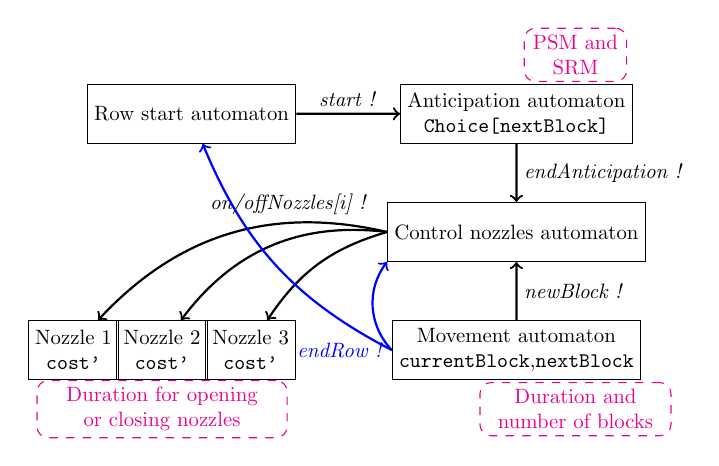
\begin{tikzpicture}[scale=.75, transform shape]
	\node[draw,minimum width=1cm,minimum height=1cm] (SA) at (-3,3) {Row start automaton};
	\node[draw,minimum width=1cm,minimum height=1cm,  align=center] (AA) at (2.5,3) {Anticipation automaton \\ \texttt{Choice[nextBlock]}};
	\node[draw,minimum width=1cm,minimum height=1cm] (CA) at (2.5,1) {Control nozzles automaton};
	\node[draw,minimum width=1cm,minimum height=1cm, align=center] (MA) at (2.5,-1) {Movement automaton \\ \texttt{currentBlock},\texttt{nextBlock}};
	\node[draw,minimum width=1cm,minimum height=1cm, align=center] (NA1) at (-5,-1) {Nozzle 1 \\ \texttt{cost'}};
	\node[draw,minimum width=1cm,minimum height=1cm, align=center] (NA2) at (-3.5,-1) {Nozzle 2 \\ \texttt{cost'}};
	\node[draw,minimum width=1cm,minimum height=1cm, align=center] (NA3) at (-2,-1) {Nozzle 3 \\ \texttt{cost'}};
	
	\draw[->,thick] (SA) to node[above]{\textit{start !}} (AA);
	\draw[->,thick] (AA) to node[right,] {\textit{endAnticipation !}} (CA);
	\draw[->,thick] (MA) to node[right]{\textit{newBlock !}} (CA);
	%\draw[->,thick] (CA) to node[right]{\textit{ON/OFF\_Nozzles}} (NA1);
	\draw[->,thick] (CA.west) to [bend right=30] node[above,pos=0.3]{\textit{on/offNozzles[i] !}} (NA1);
	\draw[->,thick] (CA.west) to [bend right=30] node[left,pos=0.4]{} (NA2);
	\draw[->,thick] (CA.west) to [bend right=20] node[left,pos=0.4]{} (NA3);
	
	\draw[->, blue, thick] (MA.west) to [bend left=20] node[left,pos=0]{\textit{endRow !}} (SA);
	\draw[->,blue, thick] (MA.west) to [bend left=40] node[left,pos=0.4]{} (CA.south west);
	
	
	\node[draw, magenta, dashed, rounded corners,text width=1.5cm, align=center] (PSM) at (3.5,4) {PSM and SRM};
	\node[draw, magenta, dashed, rounded corners,text width=3cm, align=center] (Blocks) at (3.5,-2) {Duration and number of blocks};
	\node[draw, magenta, dashed, rounded corners,text width=4cm, align=center] (Blocks) at (-3.5,-2) {Duration for opening \\ or closing nozzles};
	
\end{tikzpicture}
\caption{Scheme of our model: automata synchronisation, input data and main global variables}
\label{fig:SchemaAutomates}
\end{figure}
\vspace{-1em}
\paragraph{\textbf{Input data}}
As shown figure~\ref{fig:MethodoComplete}, the input of the models is SRM (i.e. for each block a $C_{best}$ and $C_{alt}$ command and a duration of spraying).
Each command is defined by the sets of nozzles that must be respectively opened and closed. These input data are represented in the dashed magenta nodes on figure~\ref{fig:SchemaAutomates}. They are defined in the model as command static data, implemented as global constants available for each automaton.

\paragraph{\textbf{Global variables}}
The global structure of our model is based on several global variable shared by all the automata. In particular, \texttt{currentBlock} is an integer representing the index of the vegetation block that the sprayer is currently spraying, while \texttt{nextBlock} is an integer representing the index of the next vegetation block, necessary to anticipate the opening of the nozzles. Also, the spraying command chosen by the anticipation automaton is stored in a table \texttt{Choice[]} which records the optimal command for each of the blocks.

%
\paragraph{\textbf{Synchronization between automata}} Automata can be synchronized through two types of channels: Binary channels (a transmitter and a single receiver) and Multiple channels (a transmitter and many or zero receivers). For example, in the model $PTA\_PSP$ and as shown figure~\ref{fig:SchemaAutomates}, \texttt{newBlock} is a binary channel sent at the end of each block. There are also two tables of binary channels \texttt{onNozzle} and \texttt{offNozzle}. \texttt{endRow} (to indicate the end of the row) and \texttt{endAnticipation} (to indicate that a command has been selected for the next block) are multiple channels.


\paragraph{\textbf{Modelling of the cost}} 
The quantity of sprayed product is modeled for each nozzle in the nozzles automata, using the cost rate function \texttt{cost'}. This function represents in UppAAL-CORA the flow of product sprayed at any time by the nozzle considered. The higher the flow, the higher the cost will be at the end. In UppAAL-CORA, this cost rate is an integer. The following conventions were used. When a nozzle is closed, then \texttt{cost'=0}. When a nozzle is fully opened (has normal flow) then \texttt{cost'=2}. During transitions for opening or closing a nozzle, the flow is neither zero nor maximum. These transitions are represented by a flow rate reduced by half (\texttt{cost'=1}).

\subsubsection{Verifying properties and computing the (optimal) Command Sequence}
\label{sec:VerifProp}

Specifications on the expected spraying behaviour of the Precision Spraying problem are described and formalised using UppAAL's syntax requirement specification language \footnote{https://docs.uppaal.org/language-reference/requirements-specification/} (inspired from CTL temporal logic).  

The property used to obtain the \textit{\textbf{optimal command}} sequence with the lowest cost is: \\
%\begin {description}
"Is there a command sequence that allows the sprayer to reach the end of the row (while applying the command constraints specified in the model)?" 
This property is translated in temporal logic $PP1$ by:

\textbf{PP1:} E $<>$ currentBlock == nb \_block-1\ \ and \ SA.end, 

with $SA$ is the Row start automaton, $end$ is a state in $SA$ which denotes that the sprayer reaches the end of the row and all nozzles are off, $ nb\_block$ is the number of blocks forming the row and $currentBlock$ is the block currently sprayed.
%\end {description}

The resulting command sequence can be a mixture of $C_{best}$ and $C_{alt}$ commands. It is possible to impose the use of only $C_{best}$ or $C_{alt}$ command.

% \item [only $C_{cbaset}$] $ E <> \ forall (i\ : \ int [0, nb \_block-1]) \ Choice [i] \ == \ 1 \ and \ SA.end \ $ $\rightarrow$ UPPAAL property for spraying with only $C_{best}$ used

% \item [only $C_{alt}$] $ E <> \ forall (i \ : \ int [0, nb \_block-1]) \ Choice [i] \ == \ 2 \ and \ SA.end \ $

UppAAL-CORA checks the properties and provide a trace with the lowest cost. As in the model the cost function calculates the total amount of product sprayed, the cost calculated in the optimal command is the minimum quantity of product necessary to spray the row while ensuring sufficient protection.


The model checking with the CORA function thus allows to obtain an accurate command optimising the cost criteria (here, the quantity of spraying product) while guaranteeing the correct behaviour of the sprayer. But the model checking strength can be its weakness: the enumeration of all the possible cases which guaranty the verification results also implies an intrinsic complexity. For this reason, the use of model checking on real and complex application cases is known to be difficult \cite{D2.3}. In a case such like solved here, vine rows can contain many blocks (over 100 blocks) and for each block two commands are possible. Therefore, the complexity of deciding between these two commands for each block of a row is exponential to the number of blocks.

To overcome the combinatorial explosion problem that may result from this, a decomposition methodology based on the spatial characteristic of the precision agriculture problem at hand was developed. It is described in the next section.


\section{Decomposition methodology}

The overall idea of the proposed decomposition methodology is to break down the system and/or the verification into sub-parts that can be solved independently regarding the properties to be validated over the whole system.

The hard part of the model checking decomposition is to find how to decompose while preserving a consistent expression of "local" properties with regards to the "global" ones. While the decomposition criteria provided here are specific to the Precision Spraying Problem, the intent is to propose a generic decomposition method that can be used for decision support in other agricultural domains or beyond.

The decomposition of a model checking problem should consist in three phases: the decomposition of the model (modelling decomposition), the decomposition of the verification process (verification decomposition) and the analysis of the decomposition (decomposition analysis). Modelling decomposition partitions the model into n sub-models. 2 sub-models may have an overlap zone in common and this will be detailed in section \ref{MD}.

The decomposition of verification is about decomposing the resolution of the property to be checked on the global model into the resolution of properties on the sub-models. The decomposition analysis is about proving that this verification of the properties on the sub-models guaranties the verification of the initial property on the global model.

The outline of the section follows the 3 above-mentioned phases.

\subsection{Modelling Decomposition}
\label{MD}

The modelling decomposition consists in decomposing the model into $n$ parts. One or several criteria for decomposition need to be found out in order to proceed to this.

\paragraph{\textbf{Decomposition criterion}} 

The intrinsic spatial characteristics of the agricultural applications provide guidance for decomposing. The geometrical structure of most of the agricultural fields is a useful element for decomposition. In the Precision Spraying problem, considering that each row is sprayed independently, step 3 of AMPS methodology can be applied separately to each row. The decomposition of a model including $n$ rows to $n$ models including each a unique row is thus straightforward. On the practical side, the model presented in \ref{Verif} was designed for one row, with a set of data for each row of the studied field.
Steps 1 and 2 of AMPS are better applied at a larger scale (field or vineyard) in order to have consistent crop protection of the vineyard.

Other characteristics may be used to find a decomposition criterion, depending on the application cases. The idea is to find an agricultural characteristic that imposes a fixed and known value in the verification process. This value will be the pivot of the decomposition strategy for verification.
In the Precision Spraying case, where an optimal spraying command sequence is searched, the optimal command sequence before the pivot should be independent of the optimal command sequence after it. From this idea, two criteria were identified for the Precision Spraying problem in order to decompose the verification of a row.
The first one relates to blocks with missing vegetation. The command to be applied in this case is to close all the nozzles. This criterion is close to the spatial decomposition of the different rows, as the nozzles are closed between two rows, with the significant difference that sub-systems overlap on missing vegetation blocks. The impact of overlapping will be explained hereafter.

A criterion that is more complex to handle can be extracted considering the PSM function. The presence of a block where $C_{best}$ = $C_{alt}$ in a row represents a case where the command to apply is known a priori. These blocks allow to break the dependency between the sequence of commands before and after them, which is the basic need for the decomposition process. The MC decomposition based on the criterion $C_{best}$ $=$ $C_{alt}$ is the most complex with regards to the three phases of decomposition and is detailed in the following.

\paragraph{\textbf{Forming row parts}} 
A row part is a subset of successive blocks of a row. The row parts are defined so that there is an overlapping block that belongs to two successive parts. The case considered here is the case where an overlapping block has the property that $C_{best}$ = $C_{alt}$). Such block will be called hereafter a "same command block".

Thus, a row $R$ is decomposed into $ n $ parts $ \{P_1$, ..., $P_n\}$. Each $P_i$ is a set of blocks which begins with a block where $C_{best}$ = $C_{alt}$ or with the first block of the row, and which ends with a block where $C_{best}$ = $C_{alt}$ or with the last block of the row.

The figure \ref{fig:decompo_in_two} illustrates, by an example, the formation of the row parts.

The hypothetical example row $R$ is formed of $5$ blocks. The block $\{b_{3}$ is a same command block ($C_{best}$ = $C_{alt}$). The part $P_{A}$ is made up of blocks $b_{1}$,$b_{2}$ and $b_{3}$. The part $ P_{B} $ starts from block $b_{3}$ included and contains also $b_{4}$ and $b_{5}$. $b_{3}$ is the overlapping block.

\begin{figure}[h!]
	\begin{center}
		\includegraphics[width=7.2cm]{decompo2.pdf} 
		\caption{Decomposition of row $R$ in two parts} 
		\label{fig:decompo_in_two}
	\end{center}
\end{figure} 

\textbf{Generating sub-models}. Using the $PTA\_PSP$ model for UPPAAL-CORA, the generation of the sub-models for each row part consists only in editing the input data of the model. No change is needed in the description of the automata. The global constants describing commands are updated with information related to the corresponding row part: the value of the number of blocks forming the row is replaced with the value of the number of blocks forming the part (constant \texttt{nb$\_$block}); and all the tables storing the information of these blocks will be updated with only the concerned blocks.
It is worth noting that, as the configuration of the models is based on text files, the modelling decomposition is automated. It is also important to have in mind that, because the model of a part of a row is a model of a row with a reduced number of blocks, some parts have a "virtual row ending" (part $P_A$ in figure \ref{fig:decompo_in_two}) and some have a "virtual row beginning" (parts $P_B$ in same figure). Real beginnings and endings of rows have the characteristic that all the nozzles should be off before and after spraying the row. Technically, in the model of a part of a row, this constraint is also applied to its virtual beginning and its virtual ending. The consequences of this for calculating the optimal sequence and the optimal cost for a whole row from the optimal sequences and optimal costs for the parts are analysed in section \ref{PreveComp}.


\subsection{Verification Decomposition}
\label{VD}
The verification decomposition decomposes the resolution of the property to be checked on the global model into the resolution of properties on the sub-models.

Let us recall that the property allowing to obtain the optimal command sequence applied on all the rows is the property \texttt{PP1} 
described in the section \ref{sec:VerifProp}. The verification process on the sub-models is based on the same property, but with the modifications of the models previously mentioned.

The decomposition of the verification consists in verifying this property on each row part. It is important to note that in the model of a part, $ nb\_block $ becomes the number of blocks forming the part and $ StartRowAut.end $ is reached when the sprayer finishes spraying all the blocks of the part. 

Checking the property \texttt{PP1} on the sub-model allows to calculate the Optimal Sequence to be applied on the part and to calculate its Optimal Cost. 
The complete optimal sequence can be calculated from the concatenation of the optimal sequences of the parts, and the global optimal cost can be calculated from the sum of the optimal costs of the parts. Rules for concatenation and cost rectification terms respectively required in these operations when overlapping occurs in decomposition (see figure \ref{fig:decompo_in_two}) will be explicited hereafter.

\subsection{Decomposition Analysis}
\label{PreveComp}

The decomposition analysis is about proving that the verification of the properties on the sub-models allows the verification of the initial property on the global model.
Let us consider a row, or row part such as in figure \ref{fig:decompo_in_two}, which can described by equation \ref{eq:SRExample_r}:

\begin{equation}
	S_R = \oslash \triangleright C?_{1} \triangleright C?_{2} \triangleright C_{3} \triangleright C?_{4} \triangleright C?_{5} \triangleright \oslash \label{eq:SRExample_r}
\end{equation}

In equation \ref{eq:SRExample_r}, $\oslash$ means that all nozzles are off. $C?_{i}$ denotes a choice to make for block $b_i$ and $C_{i}$ is the command for block $b_{i}$ when it has a unique possibility. The decomposition can be made here using block $b_3$ as overlapping block.  Sequences $S_A$ and $S_B$ for the resulting parts $P_A$ and $P_B$ can be written:
\begin{eqnarray}
	&S_A =& \oslash \triangleright C?_1 \triangleright C?_2 \triangleright C_{3}* \triangleright \oslash \label{eq:SAExample_r}
	\\
	&S_B =& \oslash \triangleright *C_{3} \triangleright C?_4 \triangleright C?_5 \triangleright \oslash \label{eq:SBExample_r}
\end{eqnarray}

The symbol $*$ either on the left or on the right of $C_3$ denotes that overlapping occurs here. The concatenation law for parts having an overlapping is given in equation \ref{eq:ruleconcatparts}. It can easily be shown that when applying this concatenation law to $S_A$ and $S_B$, then $S_R = S_A \triangleright S_B$.

\begin{equation}
	C* \triangleright \oslash \triangleright \oslash \triangleright *C = C \label{eq:ruleconcatparts}
\end{equation}

Now, as written in equation \ref{eq:costcorrection}, the rectification terms for calculating the cost of $S_R$ from the costs obtained for $S_A$ and $S_B$ once solved by CORA algorithm can be formulated. Considering that the cost for $C_3$ has been counted once in $S_A$ with $C_3 *$ and once again in $S_B$ with $*C_3$ then the cost $Q_{3}(C_{3})$ of this command should be retrieved from the sum of costs of parts. Considering also that there was no actual closing and re-opening of nozzles for $C_3$ between $C_3 *$ and $*C_3$, the formulation of the cost correction term is provided in equation \ref{eq:correctionterm}. This reasoning applies to any decomposition of a row in $n$ parts by simple recursion of cutting a part in two. The calculation of optimal cost of a row from optimal sequences on $n$ row parts is thus demonstrated.

\begin{equation}
	c(S_A \triangleright S_B)=c(S_A)+c(S_B)+corr(S_A \triangleright S_B) \label{eq:costcorrection}
\end{equation}
%\vspace{-1em}
\begin{equation}
	corr(S_A \triangleright S_B)= - Q_{3}(C_{3}) - close(C_{3}) - open(C_{3}) \label{eq:correctionterm}
\end{equation}

In this section, it was shown how to proceed to model-checking decomposition.
In section \ref{results}, the decomposition methodology will be applied on a real vine plot. The next section details the data acquisition system and presents the vineyard on which our precision spraying approach will be tested.





\section{LiDAR field data}
\label{lidar}


\subsection{2D LiDAR information of canopy structure}
A Sick LMS100 (SICK AG, Düsseldorf, Germany) 2D LiDAR sensor was used in the study. The LMS100 is a fully-automatic divergent laser scanner based on time-of-flight (TOF) measurement with a typical error of $\pm 30$ mm, a selectable angular resolution set to $0.5^{\circ}$, a maximum scan angle of $270^{\circ}$ and a maximum range of 20 m. With these settings, there were 541 distances recorded for each complete laser rotation, which is hereafter referred to as a “scan”, and scans were obtained at 50 Hz. The LMS100 laser emission wavelength is 905 nm (near infrared) and it is Class one eye-safe. The LMS100 and data logging system were mounted on a purposely-built stainless-steel mast fixed behind the tractor operating the sprayer, according to a previously described procedure \cite{cheraiet2020algorithm}. The LMS100 sensor height ranged from 1.1 m above ground level. The tractor was driven along the vineyard rows at a constant forward travel speed of 5 $km/h$, with a typical error of ± 0.21 $km/h$.
This sensing system was coupled to a Real Time Kinematic (RTK) GNSS receiver (Teria GSM correction, Vitry-sur-Seine, France) to identify the start and end point of the sampling units. Once the starting point was set, scans were aggregated using a fixed forward distance based on the constant tractor speed to generate a 3D point cloud reconstruction of the vine environment. %The sprayer replicated commercial operations, i.e. the tractor only traversed every second row so that the canopy was only scanned from one side. This differs from most previous research activities with LiDAR sensors, but was deliberately done to approximate commercial conditions. 
Full details of the system set-up are given in \cite{cheraiet2020algorithm}.% Cheraiet et al. (2020).

\subsection{Field data}
% ADAPTER SELON 1 ou 2 DATES 
A vine estate with one block, "Aglae" (Vitis vinifera L. cv Marselan), was chosen for the study in 2019. Located in Grabels, close to Montpellier (Hérault, France), the Mas Piquet Estate is characteristic as a vineyard from the south of France, both in terms of grape varieties and training systems. The rows were northeast-southwest oriented. Vines were trellised in 2.5 m rows with a 1.0 m vine spacing within rows using a cordon Royat system that comprised a cordon wire and at least one trellising wire. 2D LiDAR acquisitions were carried out on the date 2019/07/31 during the season. This date corresponds to the beginning of veraison (81) in BBCH scale growth stages \cite{lorenz1994phanologische}.

From the data obtained, we were able to study the dynamics at an intra-plot scale of canopy height and width. The height and width of the vegetation increased almost linearly from the flowering stage to the bunch closure stage. At the scale of the whole plot, the vegetation height was between 0.85 m and 1.64 m, and a vegetation thickness of between 0.39 m and 0.95 m. Trimming, combined with increasing water stress over summer, tends to stagnate any further growth.

In order to define vegetation states and as explained in section \ref{sec:vegcar}, some thresholds need to be set. The thresholds to separate the height sections were respectively set to $0.3$, $0.7$ and $1.1\ m $ and the maximum vine height was set to $1.7\ m $. The discrimination threshold between 1 and 2 was chosen as the median of the number of LiDAR beams
interceptions in the considered horizontal section and for the whole field. The thresholds for abstract value 0 were chosen specifically for each horizontal section: below 5 LiDAR interceptions for a 10 cm wide scan slice for H section, below 34\% of the median for M section and below 10\% of the median for L section. It is important to note that such thresholds depend on the BBCH scale growth stages, and they were defined for all rows forming the plot.   


In the following, the AMPS method and the decomposition methodology will be implemented on the study plot.


\section{RESULTS \& DISCUSSION}
\label{results}

In this section, we will apply the AMPS method for real vine LiDAR data. The optimal command sequence, taking into account sprayer dynamics, will be compared to classical spraying. \Rim{The classic spraying process is carried out using only the two hands (LH\&HH) of the sprayer without any automation during the entire spraying process.}

The AMPS step 1 consists on defining the precision spraying mapping, which maps each vegetation state to two spray commands $C_{best}$ and $C_{alt}$. We have already to provide this map in Section \ref{step1} (cf. Table \ref{tb:PSM}). Now, we proceed to apply step 2.

\subsection{Computation of blocks and spatialized recommendation map}

The AMPS step 2 consists in the processing of the LiDAR data to obtain $C_{best}$, $C_{alt}$ and the duration of each vegetation block for the studied plot. The sprayer is supposed to move at 1.4 $m/s$. The length of a block is expressed as a function of the time needed to spray it. 

\Rim{The algorithm, based on filtering and aggregation rules (see section \ref{sec:step2}), was implemented using the Pyzo IDE, a free and open-source computing environment based on Python 3\footnote{{https://pyzo.org/index.html}}}. 

The tables \ref{tb:step2Aglae}, \ref{tb:stepVegState} and \ref{tb:stepAnalysis} provide for an analysis of the algorithm and are explained and commented in the sequel.

In the table \ref{tb:step2Aglae}, the column "Row" provides an identifier to each row, this ID is a value between 1 and 5. The column "D" represents the duration of time (in s) needed to spray the row in seconds (s). The column "NB" gives the number of blocks forming the row, the column "M" provides the number of blocks with a missing vegetation and the column "NS" gives the number of blocks where the command $C_{best}$ is equal to the command $C_{alt}$. The column "$D_{max}$" (in s) provides the higher duration of a block in the row, the column " $ND_{min}$" provides the number of blocks having the smaller duration of 0.4 s in the row and the column " $NL$" provides the number of blocks having a duration longer than 1 s in the row.

\begin{table}[ht]
	\begin{center}
		\rotatebox{90}{
			\begin{tabular}{|c|c|c|c|c|c|c|c|}
				\hline 
				Row		&	D   &	NB      & M        &   NS	    & $D_{max}$  &   $N D_{min}$ & NL \\ 
				&	 (s)   &	      &         &       &  (s)  &   & \\ \hline
				1		&   40,1	&	58      &   1       &   24      &	1,7                 &     16    &9\\ \hline
				2		&	65,2    &	84      &   2       &   44     	&	2,1                 &    21     &23\\ \hline
				3	    &	67,9	&	89      &   5       &   43      &	4,6                  &    21     &15\\ \hline
				4   	&	71,2    &	82      &   5       &   42	    &	3,6                &    18     & 26\\ \hline
				5	    &	70,5    &	90      &   0       &	41	    &	5,3                &    27     &	19\\ \hline
				
		\end{tabular} }
		\caption{Row decomposition}\label{tb:step2Aglae}
	\end{center}
\end{table}

In all rows, the number of "same command" blocks \Rim{(see column "NS")} represent around 50\% of the number of blocks forming the row. This has two consequence for this particular field and date: the optimisation has an effect on approximately half of the blocks of row, and there are many blocks that can be chosen to support model decomposition for calculating optimal spraying sequences. \Rim{The number of blocks having the smaller duration of 0.4 s (see column "$ND_{min}$") represents 1/4 of the number of blocks forming the row which means that the resolution chosen is appropriate for the sprayer's dynamics. The number of blocks having a duration longer than 1 s (see column $NL$) gives an idea about homogeneous blocks and this show that the experiment was valid.}

\begin{table}[h]
	\begin{center}
		\begin{tabular}{|p{1,3 cm}|p{0,5cm}|p{0,5 cm}|p{0,5 cm}|p{0,5 cm}|p{0,5cm}|}
			\hline 
			Veg.states (THML)                & R1 	            & R2                 & R3              & R4              & R5               \\ \hline
			'x x 0 x '     & X                     & X                     & X                  & X                  & \textcolor{red}{X}  \\
			\rowcolor{yellow} '1 0 1 0 '     &                       &                       &                    & \textcolor{red}{X} &                     \\
			'1 0 1 1 '     & X                     & X                     & X                  & \textcolor{red}{X} & \textcolor{red}{X}  \\
			'1 0 1 2 '     & X                     & \textcolor{red}{X}    & \textcolor{red}{X} & \textcolor{red}{X} & \textcolor{red}{X}  \\
			'1 0 2 1 '     & X                     & \textcolor{red}{X}    &                    & X                  &                     \\
			'1 0 2 2 '     & \textcolor{red}{X}    & X                     & \textcolor{red}{X} & \textcolor{red}{X} & \textcolor{red}{X}  \\
			\rowcolor{yellow} '1 1 1 0'      & \textcolor{red}{X}    & \textcolor{red}{X}    & \textcolor{red}{X} & \textcolor{red}{X} & \textcolor{red}{X}  \\
			'1 1 1 1 '     & X                     & X                     & X                  & X                  & X                   \\
			'1 1 1 2 '     & X                     & X                     & X                  & X                  & X                   \\
			'1 1 2 0 '     & \textcolor{blue}{X}   &                       & \textcolor{red}{X} &                    &                     \\
			'1 1 2 1 '     & X                     & X                     & X                  & X                  & X                   \\
			'1 1 2 2 '     & \textcolor{red}{X}    & \textcolor{red}{X}    & \textcolor{red}{X} & \textcolor{red}{X} & \textcolor{red}{X}  \\
			\rowcolor{yellow} '1 2 1 0 '     & \textcolor{red}{X}    & \textcolor{red}{X}    & \textcolor{red}{X} & \textcolor{red}{X} & \textcolor{red}{X}  \\
			'1 2 1 1 '     & X                     & X                     & X                  & X                  & X                   \\
			'1 2 1 2 '     & \textcolor{red}{X}    & \textcolor{red}{X}    & \textcolor{red}{X} & \textcolor{red}{X} & \textcolor{red}{X}  \\
			'1 2 2 0 '     & \textcolor{red}{X}    & \textcolor{red}{X}    & \textcolor{red}{X} & \textcolor{red}{X}  &                    \\
			'1 2 2 1 '     & \textcolor{red}{X}    & \textcolor{red}{X}    & \textcolor{red}{X} & \textcolor{red}{X} & \textcolor{red}{X}  \\
			'2 0 1 2 '     & \textcolor{red}{X}    & \textcolor{red}{X}    &                    &                    &                     \\
			'2 0 2 1 '     & \textcolor{red}{X}    &                       &                    &                    & \textcolor{red}{X}  \\
			'2 0 2 2 '     & \textcolor{red}{X}    & X                     &                    & \textcolor{red}{X} &                     \\
			'2 1 1 2 '     & \textcolor{red}{X}    & X                     & X                  & X                  & X                   \\
			'2 1 2 0 '     &                       &                       &                    & \textcolor{red}{X} &                     \\
			'2 1 2 1 '     & X                     & X                     & X                  & X                  & \textcolor{red}{X}  \\
			'2 1 2 2 '     & X                     & X                     & X                  & X                  & X                   \\
			'2 2 1 0 '     &                       &                       & \textcolor{red}{X} & \textcolor{red}{X} &                     \\
			'2 2 1 1 '     & X                     & X                     & X                  & X                  & X                   \\
			'2 2 1 2 '     & X                     & X                     & X                  & X                  & X                   \\
			'2 2 2 0 '     & \textcolor{red}{X}    &                       &                    & \textcolor{red}{X} &                     \\
			'2 2 2 1 '     & X                     & X                     & X                  & X                  & X                   \\ 
			'2 2 2 2 '     & X                     & X                     & X                  & X                  & X                   \\ \hline
			
			
		\end{tabular} 
		\caption{Vegetation states distribution in row}\label{tb:stepVegState}
	\end{center}
\end{table}

The table \ref{tb:stepVegState} describes for each row the vegetation states encountered before and after applying step 2. Before step 2, states are related to vegetation slices (thin blocks) and after it, states are related to vegetation blocks of various sizes.
Some states are deleted and others are added due to the aggregation rules implemented in step 2.
Deleted states (resp. added states) are represented with cross (X) in a red color (resp. blue color). Black cross means that the vegetation state is encountered before and after applying step 2. \\
It can be seen that some vegetation states are present in all rows such as (T-H-M-L) = (1-1-1-1). The vegetation state (T-H-M-L) = (1-1-2-0) is added in the row 1 after applying $RAF1$ and some states are present in some rows and deleted after applying $RAF1$ such as (T-H-M-L) = (1-0-1-1) present in the rows 1, 2 and 3 and deleted in rows 4 and 5. This is due to the minimum size of the block. Many states that are present in slices are deleted when applying step2. Only one state is added and in only one row. \Rim{If one refers to Table \ref{tab:SRM}, the vegetation state (T-H-M-L) = (1-0-0-1) is deleted after appling step 2. It is important to note that deleted vegetation states is due to the dynamics of the sprayer, which is linked to the technology, so if the reaction time were faster, no states would be deleted.}

\begin{table}[!ht]
	\begin{center}
		\rotatebox{90}{
			\begin{tabular}{|l|l|l|l|l|l|l|l|l|l|l|l|l|l|l|l|} % 16 columns
				\hline 
				& & \multicolumn{7}{c|}{\% nb blocs} & \multicolumn{7}{c|}{\% duration} \\ \hline
				Row & Cmd & $-$ & $L$ & $C$ & $H$ & $L\&H$ & $L\&C$ & $C\&H$ & $-$ & $L$ & $C$ & $H$ & $L\&H$ & $L\&C$ & $C\&H$ \\ \hline
				$R1$ & $C_{b}$ & 1.7 & 17.2 & 43.1 & 0 & 15.5 & 5.2 & 17.2 & 2 & 17.2 & 48.6 & 0 & 13.7 & 4.5 & 14\\ \hline
				$R1$ & $C_{a}$ & 1.7 & 1.7 & 29.3 & 0 & 62.1 & 1.7 & 3.4 & 2 & 2.2 & 35.7 & 0 & 56.4 & 1.2 & 2.5 \\ \hline
				$R2$ & $C_{b}$ & 2.4 & 6.0 & 26.2 & 0 & 35.7 & 16.7 & 13.1 & 2.3 & 5.7 & 28.4 & 0 & 39.1 & 14.3 & 10.3 \\ \hline
				$R2$ & $C_{a}$ & 2.4 & 0 & 15.5 & 0 & 56.0 & 14.3 & 11.9 & 2.3 & 0 & 16.9 & 0 & 58.9 & 11.0 & 10.9 \\ \hline
				$R3$ & $C_{b}$ & 5.6 & 11.2 & 22.5 & 0 & 33.7 & 6.7 & 20.2 & 10.8 & 9.6 & 21.5 & 0 & 32.8 & 5.6 & 19.7\\ \hline
				$R3$ & $C_{a}$ & 5.6 & 0 & 16.9 & 0 & 56.2 & 13.5 & 7.9 & 10.8 & 0 & 16.3 & 0 & 55.8 & 11.0 & 6.0 \\ \hline
				$R4$ & $C_{b}$ & 6.1 & 9.8 & 24.4 & 0 & 36.6 & 11.0 & 12.2 & 11.2 & 11.2 & 23.9 & 0 & 36.7 & 9.3 & 8.7 \\ \hline
				$R4$ & $C_{a}$ & 6.1 & 0 & 15.9 & 0 & 57.3 & 13.4 & 7.3 & 11.2 & 0 & 15.3 & 0 & 56.0 & 11.4 & 6.0 \\ \hline
				$R5$ & $C_{b}$ & 0 & 6.7 & 25.6 & 0 & 34.4 & 11.1 & 22.2 & 0 & 5.4 & 23.5 & 0 & 40.3 & 12.5 & 18.3 \\ \hline
				$R5$ & $C_{a}$ & 0 & 0 & 16.7 & 0 & 62.2 & 13.3 & 7.8 & 0 & 0 & 15.2 & 0 & 67.4 & 11.1 & 6.4 \\ \hline
		\end{tabular}}
		\caption{Analysis of block commands}\label{tb:stepAnalysis}
	\end{center}
\end{table}

In table \ref{tb:stepAnalysis} are analysed the frequencies of potential commands for blocks, before choice between $C_{best}$ and $C_{alt}$ that is made at step 3. For each row and for each alternative $C_{best}$ (row $C_{b}$) or $C_{alt}$ (row $C_{a}$), the frequency of each spray command is provided, as a percentage of the number of blocks in the row and as a percentage of the duration in the row. Let us recall that from the precision sprayer mapping defined in step 1 of AMPS (cf. section \ref{step1}), 7 spray commands were considered. Their names are here abbreviated: $-$ (all nozzles off), $L$ ($LH$), $C$ ($CH$), $H$ ($HH$), $L\&H$ ($LH\&HH$), $L\&C$ ($LH\&CH$), and $C\&H$ ($CH\&HH$). The frequency for number of blocks is defined as $N/T$ where $N$ is the number of blocks having this command and $T$ is the number of blocks in the row. The frequency for duration is defined as $D/R$ where $D$ is the sum of the durations of the blocks having this command and $R$ is the duration for spraying the whole row.

The frequencies for number of blocks and durations are consistent. In 4 of the 5 rows, the most frequent preferred command is the usual $LH\&HH$ which corresponds to dense vegetation. $CH$ is also a very frequent preferred command in these rows, which allows to reduce the overall consumption of phytosanitary products when $C_{best}$ is chosen at step 3. The first row has lower vigour and the most frequent preferred command in this row is $CH$. $CH$ corresponds to spraying the whole vegetation height when lower density is present. The commands $LH$ and $HH$ are less frequent but useful. The command $HH$ does not appear in any row and any control sequence. This was expected. Indeed, from the precision spraying mapping defined in AMPS step 1, the command $HH$ appears, for the $C_{alt}$ control sequences, in the vegetation state (T-H-M-L) = (1-0-1-0) and for the $C_{best}$ control sequences, in the vegetation states (T-H-M-L) = (1-1-1-0) and (T-H-M-L) = (1-2-1-0) (cf. yellow rows in the Table \ref{tb:stepVegState}). The vegetation states in yellow cells are deleted after applying the step 2 of AMPS due to the aggregation rules. Therefore, the command $HH$ does not appear. 

The following subsection will deal with the calculation of the optimal command sequence. 

\subsection{Computation of spraying command map  using decomposition analysis}
Let us recall that the optimal command sequence is obtained by verifying property \texttt{PP1} on the $PTA\_PSP$ model using the UppAAL-CORA tool.

It was not possible to find the optimal command sequence for any row without using the decomposition method, due to the combinatorial explosion problem, which typically occurs 2 to 3 minutes after the start of the verification. Two reasons explain this combinatorial explosion: the first is related to the intrinsic complexity of model-checking. Indeed, by simplifying, if we consider only the complexity for one row which is composed, at least, of 58 blocks and for each block in this row two commands are possible, which makes a complexity of at least $2^{58}$. To find the best cost, the model checking process generates a significant part of the whole tree and it explodes. The second reason is related to a technical limitation of the UppAal-CORA model-checking tool. Indeed, the available binary of UppAAL-CORA was built only for a 32-bit architecture, which limits the memory usage to 4 GB of RAM. Computing the optimal command sequence using more than 4 GB of memory was therefore technically not possible.

To overcome the combinatorial explosion in order to be able to compute the optimal command sequence, the decomposition methodology was applied. 
\subsubsection{Modelling Decomposition}

Let us recall that the modelling decomposition consists on decomposing the row into n row parts and then, generates the sub-model associated to each part. The decomposition criterion here is $C_{best}$ = $C_{alt}$. From Table \ref{tb:step2Aglae} and in all rows, the number of blocks having the same commands (column $NS$) represents around 50\% of the number of blocks forming the row (column $NB$). Therefore, applying the decomposition criterion $C_{best}$ = $C_{alt}$ each time it happens in the sequence would produce many row parts of 2 blocks and would unnecessarily complicate the validation process. Thus, the decomposition process was arranged so that parts would have a minimum length of 25 blocks. This value was determined from expertise after calculation trials.

In the table \ref{tb:rowDec}, the column "Row" is the identifier of each row. The column "NB" gives the Number of Blocks forming the row, the column "NP" provides the Number of Parts, the column "PL" gives the Part Limits, and the column "NB\_P" provides the Number of Blocks in each Part.
\begin{table}[ht]
	\begin{center}
		\rotatebox{90}{
			\begin{tabular}{|c|c|c|c|c|} 
				
				\hline 
				R		& NB    & NP  &	PL     & NB\_P       \\ \hline
				1		& 58    & 3	   & $b_0\_b_{26}, b_{25}\_b_{51}, b_{50}\_b_{59}$	      &   26, 26, 8       \\ \hline
				2		& 84	& 4    & $b_0\_b_{26}, b_{25}\_b_{52}, b_{51}\_b_{77}, b_{76}\_b_{85}$	      & 26, 27, 26, 8          \\ \hline 
				3	    & 89	& 4	   & $b_0\_b_{27}, b_{26}\_b_{52}, b_{51}\_b_{81}, b_{80}\_b_{90} $     & 27, 26, 30, 9         \\ \hline 
				4   	& 82	& 4    & $b_0\_b_{26}, b_{25}\_b_{51}, b_{50}\_b_{76}, b_{75}\_b_{83} $	      & 26, 26, 26, 7        \\ \hline
				5	    & 90	& 4    & $b_0\_b_{27}, b_{26}\_b_{53}, b_{52}\_b_{78}, b_{77}\_b_{91} $ 	      &  27, 27, 26, 13       \\ \hline
				
		\end{tabular} }
		\caption{Row decomposition}\label{tb:rowDec}
	\end{center}
\end{table}

It can be noted that, in general, the number of blocks forming parts is between 26 and 30 blocks. The last part of each row has a small size (between 7 and 13 blocks) because it is formed by the rest of blocks forming the row.
\subsubsection{Spray savings}
In this section, the spray savings are analysed for each of the five rows. 

In the table \ref{tb:CompCost}, the column "Row" is the identifier of each row. The column "NB" gives the Number of Blocks forming the row. The column "Classical cost" gives the cost while using the classical spray configuration $LH\&HH$ for the entire row. The column "Best cost" gives the cost while using the best spray configuration $C_{best}$ thanks to the two first steps of AMPS. The column "Optimal cost" gives the cost while using the third step of the AMPS method, which computes the optimal spray configuration (a mixture of the $C_{best}$ and $C_{alt}$ commands). %We provide between brackets the number of times that $C_{Calt}$ is used in the optimal configuration ($N_{Calt}$).  
%3,7 row 1 - 28,4 %
%4,2 row 2 - 14 %
%3,1 row 3 - 20,6
%2 row 4 - 23, 6
%2 row 5 - 9,6%
\begin{table}[ht]
	\begin{center}
		\begin{tabular}{|c|c|c|c|c|}
			\hline 
			Row		& NB  		&	Classical   &	Best    &  Optimal      \\
			&   		&	 cost  &	 cost   &   cost     \\ \hline
			1		& 58		&   1604        	&	1192        &   1148           \\ \hline
			2		& 84		&	2608            &	2344        &   2244              \\ \hline
			3	    & 89	    &	2716        	&	2226        &   2156              \\ \hline
			4   	& 82    	&	2848            &	2220        &   2176            \\ \hline
			5	    & 90	    &	2820            &	2596        &   2548            \\ \hline
		\end{tabular} 
		\caption{Comparative spraying configurations}\label{tb:CompCost}
	\end{center}
\end{table}

The optimal cost is the lowest in the Table \ref{tb:CompCost}. It provides a saving of 2\% to 4 \% with reference to a sequence choosing always $C_{best}$ (best cost) and a saving of 10\% to 28 \% with reference to classical spraying (constant $LH\&HH$, which requires no automation). The saving between best cost and optimal cost is small in this example. This is due to the number of blocks having the same commands which represents around 50\% of the number of blocks forming the row.


Besides performances of the approach on the specific example provided, the interest of the AMPS method is its genericity (the same model can be used for the verification of several properties) and its capacity to manage complexity (dealing with the combinatorial explosion problem using the decomposition methodology). 

\section{Conclusion} 

This paper dealt, in the context of the phytosanitary treatment of vineyards, with the issue of discrete control sequences for variable rate application in precision agriculture. The objective was to handle the dynamics of sprayer nozzles dynamic so that two objectives can be simultaneously achieved: getting sufficient protection on each plant and reducing overall the use of the phytosanitary products in the field. Based on model checking and Cost Optimal Reachability Analysis, this paper proposed a complete method to address this objective in which accuracy, optimality and complexity issues are handled.

The proposed Automata Modelling for Precision Spraying (AMPS) method is decomposed in 3 main steps. The preliminary phase catches the human expertise and defines the links between the best ($C_{best}$), the alternative appropriate ($C_{alt}$) sprayer commands and the vegetation density to obtain an accurate and acceptable protection. Step 2 performs aggregation of raw LiDAR data to obtain manageable density characteristics of vine rows as a sequence of vegetation blocks to which can attached  possible commands for nozzles, with a preferred and an alternative command for each block. Finally, from Priced Timed Automata modelling that represent the sprayer movement inside a row and the functioning of nozzles, step 3 uses model checking and the UppAAL-CORA tool to compute the optimal and accurate sequence to spray a row with a minimal quantity of phytosanitary product.

In addition, to address real vineyard applications and deal with the problem of combinatorial explosion of the state-space, a decomposition method of the model-checking analysis was proposed. 

The limitations of this reseach may be analysed in order to identify further research needs:
\begin{itemize}
	\item Genericity: the paper was written with an example of possible spraying technology. It can be easily extended to actual and various sprayer types of today and of the future. The control method proposed here allows to handle sets of nozzles which would have overlapping sprays, in order to precisely target the vegetation to protect.
	\item Ergonomic design of decision-support: it is clear that the tooling used in this paper is not fit for a direct use by farmers. The AMPS method was implemented in a software tool that can automatically generate an optimal spraying command from LIDAR Data using the current model of an imaginary sprayer. A flexible and adaptable human-machine interface should now be developed to facilitate the dialogue with the end-user and for modelling various sprayers. An alternative to the development of a customisable tool would be that a manufacturer of a variable rate sprayer would model it and propose a decision system based on field data.
	\item Consideration of new spraying criterion: 2 criteria were considered in this paper: the accuracy and the optimality of the command. The quality of spraying is implicitly represented in the paper by $C_{best}$ and $C_{alt}$ configurations. Quality could be  quantified and be the subject of optimisation.
	\item MC analysis performance: the paper is based on UppAAL-CORA tool. There are alternatives to UppAAL for modelling timed systems and temporal issues. Yet, available tools for performing CORA analysis are limited. Implemeting CORA features in other model-checkers would allow to compare performances and select tooling that best minimises computation time and/or the amount of the required hardware memory.
\end{itemize}

Other questions concerning precision agriculture could be treated using model checking.

Furthermore, model checking can also be useful to optimize the control of an agricultural robot or a multi-robot team, or to ensure their safety or security.

\bibliographystyle{elsarticle-num}  
\bibliography{bib.bib}


\appendix
\newpage

\section{Detailed description of $PTA\_PSP$ model}
\label{AnnexeModeles}
In this annex, we proposed a detailed description of each automaton that is part of the model $PTA\_PSP$. Let us recall that $PTA\_PSP$ model is composed of 7 Priced Timed Automata:
\begin{itemize}
	\item \texttt{Row start automaton (SA)}: manages the starting of spray in the row,
	\item \texttt{Movement automaton (MA)}: manages the movements of the sprayer inside the row from block to block,
	\item \texttt{Anticipation automaton (AA)}: selects the spraying command for the next vegetation block,
	\item \texttt{Control nozzles automaton (CA)}: manages the opening and closing of each nozzle according to the chosen spraying command,
	\item \texttt{Nozzles automata (NA$_i$)}: represent the behaviour of each nozzle (3 nozzles represented by 3 automata).
\end{itemize}

\subsection{\textbf{Row start automaton (SA)}}
This automaton, represented in the figure \ref{fig:start}, manages the startup phase. It sends a command event $"start0"$ to the \textit{anticipation automaton} to select a command for the first block. When selection is finished, it receives from the \textit{anticipation automaton}, a $"finishAnticipation"$ event. Then, it sends $"start1"$ event to the \textit{nozzle control automaton} to activate the nozzles for the first block. It waits $max\_temp\_open\_Nozzle$ the time required for nozzles to be opened. It sends to the \textit{movement automaton} a $"new \_block" $ event to start spraying at the first block. When spraying is finished it receives an $"endRow"$ event. When all nozzles are closed ($allClose == true$), it passes to the state $end$.

\begin{figure} [h!]
	\begin{center}
		\includegraphics[width = 8cm]{Vegetation.pdf}
		\caption{Row Start automaton} \label{fig:start}
	\end{center}
\end{figure}


\subsection{\textbf{Anticipation automaton.}} This automaton, represented in the figure \ref{fig:ant}, makes it possible to select a command for the following block. The two possible commands for each vegetation block are $ C_ {best} $ and $ C_ {alt} $ which are stored respectively in $ CBest $ and $ CAlt $. \textit{The anticipation automaton} first receives the signal $"start0"$ from \textit{the Row Start automaton}. Then, if the value of the variable $ Choice $ is -1 (choice not predefined) then it chooses an order from $ CBest $ and $ CAlt $, stores its choice in the variable $ Choice $ and calls the function $ updateNextNozzle $. If $ Choice $ is predefined, then this choice is followed. Finally, \textit{the anticipation automaton} sends, in broadcast, the event $"finishAnticipation"$ and updates the variable $anticipe$ to \texttt{false} so as not to loop indefinitely.


\begin{figure}[h!]
	\begin{center}
		\includegraphics[width=9cm]{Anticipation.pdf}
		\caption{Anticipation automaton} 
		\label{fig:ant}
	\end{center}
\end{figure}

\subsection{\textbf{Movement automaton.}} This automaton, represented on the figure ~\ref{fig:dep}, allows to represent the movement of the sprayer. The time required to spray a vegetation block is computed in step 2, based on the length of the block and the speed of the sprayer. This information is stored in the $ tempo\_block $ variable. At the start,the sprayer is in the $"Init"$ state. When it receives the start event $"new\_block"$, it goes to the state $ block $. The state $ block $ has an invariant $ t\_block <= tempo\_block [currentBlock] $, the sprayer remain in this state for the duration of this block. The state $ block $ has also a guard $ t\_block == tempo\_block [currentBlock ] $ on its outgoing transitions, the automaton signals the end of a block by sending in broadcast the event $"new\_block"$ and the end of a row by sending in broadcast the event $"endRow"$ (it then returns to the state $ Init $).
\begin{figure}[h!]
	\begin{center}
		\includegraphics[scale=0.6, angle =90 ]{dep.pdf}
		\caption{Movement automaton} 
		\label{fig:dep}
	\end{center}
\end{figure}

\subsection{\textbf{Nozzles automata.}} These automata represent the behavior of each nozzle (figure \ref{fig:nozzle}). Each of these automata has four states: $OFF$ (initial state), $ON$, $TransitionOfOpen$ (opening) and $TransitionOfClose$ (closing). It receives the signals $"onNozzle"$ and $"offNozzle"$ to pass from a state to another. 
The nozzles response time, for opening or closing, is supposed to be a fixed and known ($ max \_temp\_open\_Nozzle $, $ max\_temp\_close\_Nozzle $). It is set at 0.2s in our example.

\begin{figure}[ht!]
	\begin{center}
		\includegraphics[scale = 0.8, angle =90]{nozzle.png}
		\caption{Nozzles automata} 
		\label{fig:nozzle}
	\end{center}
\end{figure}

\subsection{\textbf{Control Nozzles automaton.}} The role of this automaton, described in figure \ref{fig:CtrNozzle}, is to control the nozzles. When it receives the signal $ "finishAnticipation"$ from \textit{the Anticipation automaton}, it calls the function $control ()$ which determines the nozzles to be opened or closed for the next block. To secure the quantity of sprayed product in each block, the nozzles selected for opening are opened 0.2s before the start of the block (the value 0.2 is stored in the constant $ max\_temp\_open\_Nozzle $). Conversely, those which must be closed will not be completely closed until 0.2s after the block change (the value 0.2 is stored in the constant $ max\_temp\_close\_Nozzle $). To open a nozzle i, the \textit{nozzle control automaton} sends, 
$max\_temp\_open\_Nozzle $ before the end of the current block, the event $onNozzle [i]$  (see guard $t\_block <= tempo\_block[currentBlock]\-\ max\_temp\_open\_Nozzle $), and to close the nozzle i, it sends the event $offNozzle [i]$, after having received the synchronization event $new\_block$ from \textit{the movement automaton}. As soon as the commands on the nozzles are effective, then the variable $anticipe$ is set to $ True $ to allow anticipation for the next block.


\begin{figure}[h!] 
	\begin{center}
		\includegraphics[scale = 0.7]{ControlBuse.png}
		\caption{Control Nozzles automaton} 
		\label{fig:CtrNozzle}
	\end{center}
\end{figure}

\newpage

\section{Details on decomposition analysis}
The decomposition analysis is about proving that the verification of the properties on the sub-models allows the verification of the initial property on the global model. 

The idea of the proof will be illustrated on a row composed of 5 blocks, named $b_1$ to $ b_5 $, as shown in figure~\ref{fig:decompooA}. The duration of each block is greater than the sum of the opening and closing times of the nozzles, which is a necessary assumption given in the step 2 of AMPS. The row is divided into 2 parts: $ P_A $ groups together the first three blocks, and $ P_B $ includes the blocks $ b_3 $ to $ b_5 $. $b_{3}$ is the overlapping block and so is included in both $P_A$ and $P_B$. The decomposition criterion is such that $C_{best}=C_{alt}$. Thus, on the block $b_3$ for which overlapping occurs, the command is known.


\begin{figure}[h!]
	\begin{center}
		\includegraphics[width=7.2cm]{decompo2.pdf} 
		%\caption{Illustration of the proof of decomposition}
		\caption{Illustration of the decomposition to support proof} 
		\label{fig:decompooA}
	\end{center}
\end{figure} 

For the example row $R$ depicted in figure \ref{fig:decompooA}, a sequence $S_R$ for the whole row can be written:
\begin{equation}
	S_R = C?_{1} \triangleright C?_{2} \triangleright C_{3} \triangleright C?_{4} \triangleright C?_{5}  \label{eq:SRExampleA}
\end{equation} % instead of cmd_{i} 

where $C_{i}$ is the command for block $b_{i}$ when it is unique (as for the overlapping block $b_3$) and where $C?_{i}$ denotes a choice to make for block $b_i$

In order to take into account that, before each row, and at the end of each row, all nozzles should be closed, equation \ref{eq:SRExampleA} rewrites, with $\oslash$ meaning all nozzles off:

\begin{equation}
	S_R = \oslash \triangleright C?_{1} \triangleright C?_{2} \triangleright C_{3} \triangleright C?_{4} \triangleright C?_{5} \triangleright \oslash \label{eq:SRExample_r_anxA}
\end{equation}

Sequences $S_A$ and $S_B$ for parts $P_A$ and $P_B$ can be written:

\begin{eqnarray}
	&S_A =& \oslash \triangleright C?_1 \triangleright C?_2 \triangleright C_{3}* \triangleright \oslash \label{eq:SAExample_r_anxA}
	\\
	&S_B =& \oslash \triangleright *C_{3} \triangleright C?_4 \triangleright C?_5 \triangleright \oslash \label{eq:SBExample_r_anxA}
\end{eqnarray}

The symbol $*$ either on the left or on the right of $C_3$ denotes that overlapping occurs here. 

Details on the costs (product consumed) need now to be given. A rule was enunciated in section \ref{sec:Spraying_Constraints} which can be rephrased in the following way. When changing from one block to another, opening the nozzles needed in the new block and which were closed before has to be anticipated in the end of the previous block. Conversely, the nozzles no longer needed in the new block will be closed at the beginning of the new block. The consequences of this rule were explained in figure \ref{fig:CbestCalt} and section \ref{sec:InterestCalt}. The costs  for opening a nozzle $X$ ($Open(X)$), using a nozzle $X$ on a bloc $b_i$ ($Q_i(X)$), and closing a nozzle $X$ ($Close(X)$) were also introduced in section \ref{sec:InterestCalt}.

Let now $C_i$ be a command used for a block $b_i$ which can be defined as a set of opened nozzles. This set $C_i$ is any subset of $\Omega=\{LH,CH,HH\}$ with a cardinal inferior or equal to 2, including the null set $\emptyset$ (for missing vegetation blocks and outside rows).

The cost $Q_i(C_i)$ of using the nozzles of command $C_i$ during block $b_i$ can be written:
\begin{equation}
	Q_i(C_i)=\sum\limits_{X \in C_i} Q_i(X)
\end{equation}

The cost $c(C_i,C_j)$ of changing from one command $C_i$ to a command $C_j$ in the next block may be decomposed in:

\begin{eqnarray*}
	c(C_i,C_j)=open(C_i,C_j)+close(C_i,C_j)\\
	open(C_i,C_j)\ \ = \sum\limits_{X \in Cj\backslash C_i \cap C_j} Open(X) \\
	close(C_i,C_j) = \sum\limits_{X \in Ci\backslash C_i \cap C_j} Close(X)
\end{eqnarray*}

Costs of sequences can now be calculated. The cost $c(S)$ of a sequence $S= C_{i-1} \triangleright C_i \triangleright C_{i+1}$ is the following: 
\begin{equation}
	c(S)=Q_{i-1}(C_{i-1})+c(C_{i-1},C_i)+Q_i(C_i)+c(C_i,C_{i+1})\\+Q_{i+1}(C_{i+1})
\end{equation}

The costs for the start ($\alpha = \oslash \triangleright C$) and the end ($\omega = C \triangleright \oslash$) of a part or of a row are:

\begin{eqnarray}
	c(\alpha) = open(C) + Q(C) \label{eq:costalphaA}
	\\
	c(\omega) = Q(C) + close(C) \label{eq:costomegaA}
\end{eqnarray}

The concatenation law for parts having an overlapping and the rectification terms for costs of concatenated parts can now be formulated. Considering the example of figure \ref{fig:decompooA} and the sequences provided in equations \ref{eq:SRExample_r_anxA}, \ref{eq:SAExample_r_anxA} and \ref{eq:SBExample_r_anxA}, it follows that:

\begin{equation}
	S_R = S_A \triangleright S_B \Rightarrow C_{3}* \triangleright \oslash \triangleright \oslash \triangleright *C_{3} = C_{3} \label{eq:concatparts_anxA}
\end{equation}

\paragraph{Concatenation rule for row parts} Considering two row parts overlapping on a block for which command $C$ is known a priori (because $C_{best}=C_{alt}$), the concatenation rule for handling the overlapping block is the one of equation \ref{eq:ruleconcatpartsA}

\begin{equation}
	C* \triangleright \oslash \triangleright \oslash \triangleright *C = C \label{eq:ruleconcatpartsA}
\end{equation}

Considering that there is overlapping at block $b_{3}$ for which command should not be counted twice, and that termination $oslash$ of part $S_A$ and beginning $oslash$ of part $S_A$ are virtual, the concatenation rule stipulated in equation \ref{eq:ruleconcatpartsA} is easily understood.

In order to prove that the concatenation of two optimal sequences found for the parts provided by decomposition of this example is an optimal sequence for the whole row, it is required that no term should be changed in the concatenated sequence for it to be optimal, and it is required to be able to calculate the optimal cost for the whole sequence from the optimal costs of the parts.
Considering the first point, and considering two overlapping sequences such as $S_A$ and $S_B$ from our example. In an optimal choice for $C?_{1}$ and $C?_{2}$ within $S_A$, these choices only depend on the value of $C_{3}$ which is known. The same applies to choices for $C?_{1}$ and $C?_{2}$ within $S_R$. Thus, the optimal choices for $C?_{1}$ and $C?_{2}$ made in solving $S_A$ are still valid for $S_R$. With similar reasoning, it follows that optimal choices for $C?_{4}$ and $C?_{5}$ made when solving $S_B$ are still valid for $S_R$. Thus, provided that the concatenation rule stipulated in equation \ref{eq:ruleconcatpartsA} is applied, the optimal sequence for $S_R$ can be calculated from its $S_A$ and $S_B$ parts. This reasoning extends straightforwardly to calculating the optimal sequence for a vine row using $n$ row parts.
Considering the second point, cost calculation, it can be done from the costs calculated for the parts.

%\begin{equation}
\begin{eqnarray}
	c(S_A) & = & open(C?_{1})+Q_{1}(C?_{1})+c(C?_{1},C?_{2})+Q_{2}(C?_{2})+c(C?_{2},C_3) \nonumber \\*
	& + & Q_{3}(C_{3})+close(C_{3}) \label{eq:costsa_anxA} \\
	c(S_B) & = & open(C_{3})+Q_{3}(C_{3})+c(C_{3},C?_{4})+Q_{4}(C?_{4})+c(C?_{4},C?_{5}) \nonumber \\*
	& + & +Q_{5}(C?_{5})+close(C_{5}) \label{eq:costsb_anxA}
\end{eqnarray}
%\end{equation}

The cost $c(S_R)=c(S_A \triangleright S_B$) can be calculated from the $S_R$ in a similar manner as in equations \ref{eq:costsa_anxA} and \ref{eq:costsb_anxA}. Defining $corr(S_A \triangleright S_B)$ by equation \ref{eq:costcorrection_anxA}, this term can be easily calculated from equation \ref{eq:correctionterm_anxA}

\begin{equation}
	c(S_R)=c(S_A \triangleright S_B)=c(S_A)+c(S_B)+corr(S_A \triangleright S_B) \label{eq:costcorrection_anxA}
\end{equation}

\begin{equation}
	corr(S_A \triangleright S_B)= - Q_{3}(C_{3}) - close(C_{3}) - open(C_{3}) \label{eq:correctionterm_anxA}
\end{equation}

This cost correction easily extends to cost correction for the calculation of optimal cost of a row from optimal sequences on $n$ row parts.



%% If you have bibdatabase file and want bibtex to generate the
%% bibitems, please use
%%


%% else use the following coding to input the bibitems directly in the
%% TeX file.

% \begin{thebibliography}{00}

% %% \bibitem{label}
% %% Text of bibliographic item

% \bibitem{}

% \end{thebibliography}
\end{document}
\endinput
%%
%% End of file `elsarticle-template-num.tex'.
